
\section{Auswertung}
\label{sec:auswertung}
\subsection{Verifikation der Linsengleichung}
\label{sec:auswertung1}
Die Ergebnisse der ersten Messung sind in Tabelle \ref{tab:M1} aufgetragen.
\begin{table}[hp]
	\begin{minipage}{0.49\textwidth}
		\centering
		\begin{tabular}{S[table-format=3] S[table-format=3] S[table-format=3.2]}
			\toprule
			\multicolumn{3}{c}{Linse mit $\tilde{f}=\SI{100}{\milli\meter}$}\\
			%\multicolumn{3}{c}{f_1=100\,\si{\milli\meter}} & \multicolumn{3}{c}{f_2=50\,\si{\milli\meter}} \\
			{$g_1/\:\si{\milli{\meter}}$} & {$b_1/\:\si{\milli{\meter}}$} & {$f_1/\:\si{\milli{\meter}}$} \\	
			\midrule
			120 & 525 & 97.67\\
			130 & 390 & 97.50\\
			140 & 319 & 97.30\\
			150 & 277 & 97.31\\
			160 & 251 & 97.71\\
			170 & 227 & 97.20\\
			180 & 204 & 95.63\\
			190 & 198 & 96.96\\
			200 & 192 & 97.59\\
			210 & 186 & 98.64\\
			220 & 177 & 98.09\\
			\bottomrule
			\end{tabular}
	\end{minipage}
	\begin{minipage}{0.49\textwidth}
		%\centering
		\begin{tabular}{S[table-format=3] S[table-format=3] S[table-format=3.2]}
			\toprule
			\multicolumn{3}{c}{Linse mit $\tilde{f}=\SI{50}{\milli\meter}$}\\
			%\multicolumn{3}{c}{f_1=100\,\si{\milli\meter}} & \multicolumn{3}{c}{f_2=50\,\si{\milli\meter}} \\
			{$g_2/\:\si{\milli{\meter}}$} & {$b_2/\:\si{\milli{\meter}}$} & {$f_2/\:\si{\milli{\meter}}$}\\	
			\midrule
				60  & 270 & 49.1 \\
				70  & 157 & 48.4 \\
				80  & 121 & 48.2 \\
				90  & 104 & 48.2 \\
				100 &  92 & 47.9 \\
				110 &  87 & 48.6 \\
				120 &  80 & 48.0 \\
				130 &  77 & 48.4 \\
				140 &  75 & 48.8 \\
				150 &  72 & 48.2 \\
			\bottomrule
			\end{tabular}
		\end{minipage}
	\caption{Messung der Bildweiten $b_i$ bei festgelegter Gegenstandsweite $g_i$ sowie die daraus berechneten Brennweiten nach der Linsengleichung.}
	\label{tab:M1}
\end{table}
Für die berechnete Brennweite der Linsen ergeben sich Werte von 
\begin{align}
	f_1 &= \SI{97.5(2)}{\milli\meter}\\
	f_2 &= \SI{48.4(1)}{\milli\meter}.
\end{align}
Das $b$-$g$-Diagramm \ref{fig:bgdiagramm} zeigt dadurch, dass sich die Linien auf einem kleinen, nahezu punktförmigen Gebiet untereinander schneiden, die verhältnismäßig hohe Präzession der Messergebnisse an.
Des Weiteren bestätigt die Lage des Schnittpunktes mit den abgeschätzen Koordinaten $(f_1|f_1)$ respektive $(f_2|f_2)$ die Messergebnisse für die Brennweiten $f$.
Die Berechung ist somit plausibel.
Die Mittelwerte weichen von der Herstellerangabe um 
\begin{align}
	\mathup{\Delta}f_1 &= 2.5\% \quad\text{und}\quad\mathup{\Delta}f_2 = 3.2\%
\end{align}
ab.
Daher ist für die verwendeten Linsen die Brennweite $f$ über die Linsengleichung \eqref{eq:linsengleichung} verifizierbar.
\begin{figure}[hb] %% b-g-Diagramm
	\centering
	\begin{subfigure}{0.9\textwidth}
	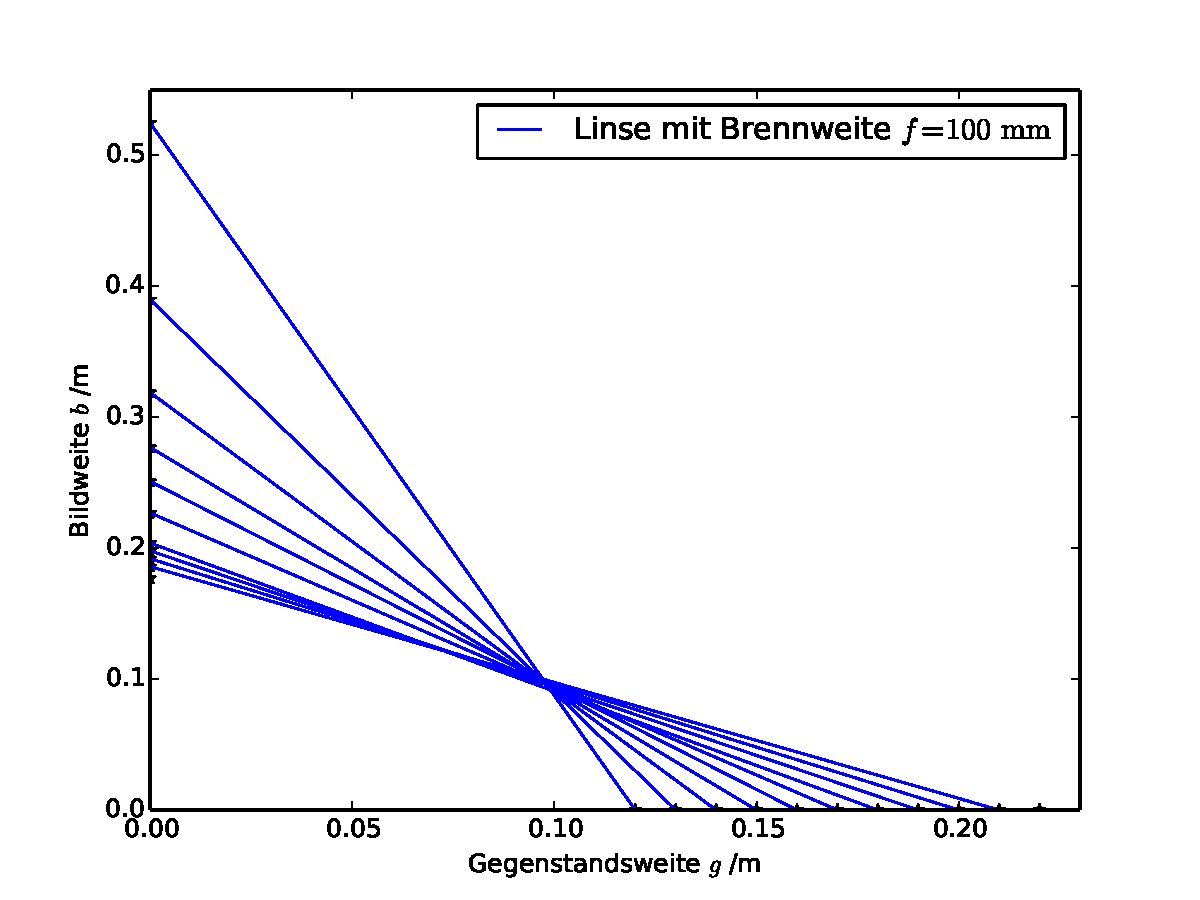
\includegraphics[width=\textwidth]{Bilder/Messung1.pdf}
	\end{subfigure}
	\begin{subfigure}{0.9\textwidth}
	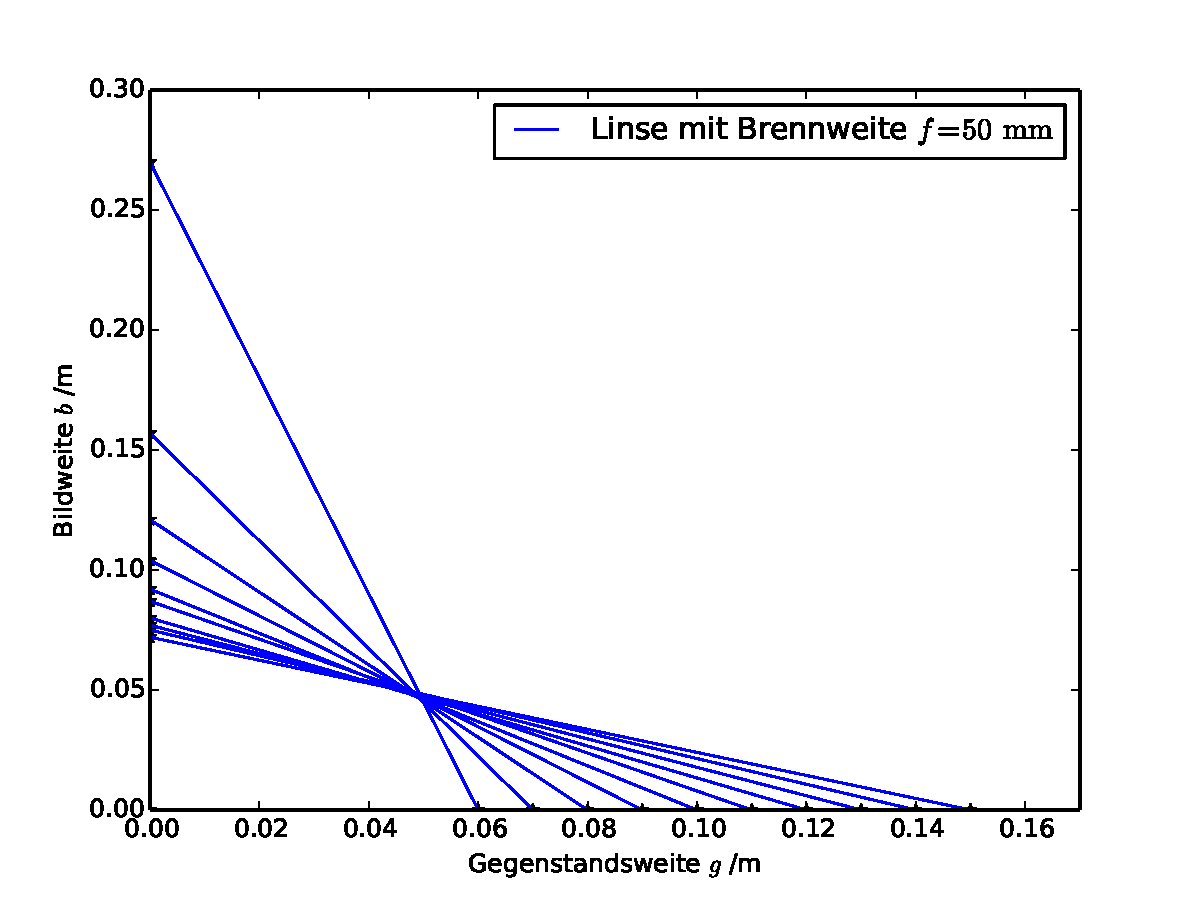
\includegraphics[width=\textwidth]{Bilder/Messung2.pdf}
	\end{subfigure}
	\caption{$b$-$g$-Diagramme zur Darstellung der Messgenauigkeit. \cite{matplotlib}}
	\label{fig:bgdiagramm} 
\end{figure}
\newpage
\subsection{Methode nach \texorpdfstring{\textsc{Bessel}}{Bessel}}
\label{sec:auswertung2}
Die Ergebnisse der Messung nach dem \texorpdfstring{\textsc{Bessel}}{Bessel}-Verfahren sind in Tabelle \ref{tab:M2} aufgetragen.
\begin{table}[htp]
	\centering
	\begin{tabular}{S[table-format=3.0] S[table-format=2.1] S[table-format=2.1] S[table-format=3.2] S[table-format=2.1] S[table-format=2.1] S[table-format=3.2]}
	\toprule
	{Abstand} &\multicolumn{3}{c}{Linsenposition 1} & \multicolumn{3}{c}{Linsenposition 2} \\
		{$e/\:\si{\milli{\meter}}$} & {$g_1/\:\si{\milli{\meter}}$} & {$b_1/\:\si{\milli{\meter}}$} & {$f_1/\:\si{\milli{\meter}}$} & {$g_2/\:\si{\milli{\meter}}$}  & {$b_2/\:\si{\milli{\meter}}$} & {$f_2/\:\si{\milli{\meter}}$}\\	
		\midrule
		450 & 144 & 306 & 97.9 &  142 & 308 & 97.2 \\
		500 & 134 & 366 & 98.1 &  135 & 365 & 98.6 \\
		550 & 127 & 423 & 97.7 &  127 & 423 & 97.7 \\
		600 & 122 & 478 & 97.2 &  123 & 477 & 97.8 \\
		650 & 119 & 531 & 97.2 &  120 & 530 & 97.8 \\
		700 & 118 & 482 & 127.7 & 117 & 583 & 97.4 \\
		750 & 116 & 734 & 60.2 &  115 & 735 & 59.4 \\
		800 & 114 & 688 & 97.8 &  116 & 688 & 99.1 \\
		850 & 114 & 736 & 98.7 &  114 & 736 & 98.7 \\
		900 & 113 & 787 & 98.8 &  113 & 788 & 98.4 \\
			\bottomrule
		\end{tabular}
	\caption{Messung der Projektionsweiten $b_i$ und $g_i$ bei festgelegtem Abstand $e$ nach \texorpdfstring{\textsc{Bessel}}{Bessel}; weißes Licht.}
	\label{tab:M2}  %% Weißes Licht, Bessel
\end{table}
Für die Brennweiten ergeben sich Werte für die beiden Linsenpositionen von 
\begin{alignat}{3}
	f_\text{Pos.1} = \SI{97(5)}{\milli\meter} \quad\text{und} \quad f_\text{Pos.2}= \SI{94(4)}{\milli\meter}.
\end{alignat}
Die gemessene Brennweite weicht in Abhängigkeit von der Linsenposition geringfügig ab,
die Schwankungen sind als statistische Fehler zu bewerten.
Der Mittelwert
\begin{equation}
	f = \SI{96(3)}{\milli\meter}
\end{equation}
zeigt eine Abweichung von der Herstellerangabe von $4\%$.

Die Ergebnisse der Messung mit einfarbigem Licht sind in den Tabellen \ref{tab:M2a} und \ref{tab:M2b} aufgetragen.
Die ermittelten Brennweiten in Abhängigkeit von der Linsenposition betragen
\begin{subequations}
	\begin{alignat}{3}
		f_\text{Rot, Pos.1} &= \SI{97.9(5)}{\milli\meter} &\qquad &&f_\text{Rot, Pos.2} &= \SI{97.3(2)}{\milli\meter}
	\end{alignat}
	\begin{equation}
		f_\text{Rot} = \SI{97.6(3)}{\milli\meter}
	\end{equation}
	\begin{alignat}{3}
		f_\text{Blau, Pos.1} &= \SI{98.2(2)}{\milli\meter} &\qquad &&f_\text{Blau, Pos.2} &= \SI{97.2(2)}{\milli\meter}
	\end{alignat}
	\begin{equation}
		f_\text{Blau} = \SI{97.7(2)}{\milli\meter}
	\end{equation}
\end{subequations}
und zeigen damit die Abhängigkeit der Brennweite von der Wellenlänge des Lichtes.
Auch hier wird sichtbar, dass die errechneten Brennweiten von der Linsenposition abhängen; 
die Schwankungen sind aber als statistische Fehler zu bewerten.
\begin{table}[p]
		\centering
		\begin{tabular}{S[table-format=2.0] S[table-format=3.0] S[table-format=3.0] S[table-format=3.2] S[table-format=3.0] S[table-format=3.0] S[table-format=3.2] }
		\toprule
			{Abstand}&\multicolumn{3}{c}{Linsenposition 1} & \multicolumn{3}{c}{Linsenposition 2} \\
			{$e/\:\si{\milli{\meter}}$} & {$g_{1,\mathup{r}}/\:\si{\milli{\meter}}$} & {$b_{1,\mathup{r}}/\:\si{\milli{\meter}}$} & {$f_{1,\mathup{r}}/\:\si{\milli{\meter}}$} & {$g_{2,\mathup{r}}/\:\si{\milli{\meter}}$} & {$b_{2,\mathup{r}}/\:\si{\milli{\meter}}$} & {$f_{2,\mathup{r}}/\:\si{\milli{\meter}}$} \\	
			\midrule
			450 & 143 & 307 & 97.6 & 306 & 144 & 97.9 \\
			550 & 126 & 424 & 97.1 & 424 & 126 & 97.1 \\
			650 & 118 & 532 & 96.6 & 531 & 119 & 97.2 \\
			750 & 117 & 633 & 98.7 & 636 & 117 & 97.7 \\
			850 & 115 & 735 & 99.4 & 739 & 111 & 96.5 \\
			\bottomrule
			\end{tabular}
			\caption{Messung der Projektionsweiten $b_i$ und $g_i$ bei festgelegtem Abstand $e$ nach \texorpdfstring{\textsc{Bessel}}{Bessel}; rotes Licht.}
			\label{tab:M2a} %% Farbiges Licht, Bessel
\end{table}
\begin{table}[p]
			\centering
			\begin{tabular}{S[table-format=2.0] S[table-format=3.0] S[table-format=3.0] S[table-format=3.2] S[table-format=3.0] S[table-format=3.0] S[table-format=3.2] }
			\toprule	
				{Abstand} &\multicolumn{3}{c}{Linsenposition 1} & \multicolumn{3}{c}{Linsenposition 2} \\
				{$e/\:\si{\milli{\meter}}$} & {$g_{1,\mathup{b}}/\:\si{\milli{\meter}}$} & {$b_{1,\mathup{b}}/\:\si{\milli{\meter}}$} & {$f_{1,\mathup{b}}/\:\si{\milli{\meter}}$} &{$g_{2,\mathup{b}}/\:\si{\milli{\meter}}$}  & {$b_{2,\mathup{b}}/\:\si{\milli{\meter}}$} & {$f_{2,\mathup{b}}/\:\si{\milli{\meter}}$}\\	
				\midrule
				500 & 366 & 134 & 98.1 & 132 & 368 & 97.2\\
				600 & 477 & 123 & 97.8 & 122 & 478 & 97.2\\
				700 & 582 & 118 & 98.1 & 116 & 584 & 96.8\\
				800 & 684 & 116 & 99.1 & 114 & 686 & 97.8\\
				900 & 788 & 112 & 98.1 & 111 & 789 & 97.3\\
				\bottomrule
			\end{tabular}
			\caption{Messung der Projektionssweiten $b_i$ und $g_i$ bei festgelegtem Abstand $e$ nach \texorpdfstring{\textsc{Bessel}}{Bessel}; blaues Licht.}
			\label{tab:M2b}
\end{table}

\subsection{Methode nach \texorpdfstring{\textsc{Abbe}}{Abbe}}
\label{sec:auswertung3}
\begin{table}[h]
	\centering
	\begin{tabular}{S[table-format=3.0] S[table-format=3.0] S[table-format=2.0] S[table-format=1.2]}
	\toprule
	\multicolumn{4}{c}{Linsensystem}\\
		 {$g'/\:\si{\milli\meter}$} & {$b'/\:\si{\milli{\meter}}$} & {$B/\:\si{\milli{\meter}}$} & {$V/\:\si{\milli{\meter}}$}\\	
		\midrule
		200 & 790 & 80 & 2.67\\
		250 & 551 & 44 & 1.47\\
		300 & 480 & 31 & 1.03\\
		350 & 416 & 25 & 0.83\\
		400 & 398 & 20 & 0.67\\
		450 & 380 & 17 & 0.57\\
		500 & 370 & 15 & 0.50\\
		550 & 346 & 13 & 0.43\\
		600 & 348 & 11 & 0.37\\
		650 & 336 & 11 & 0.37\\
	\bottomrule
	\end{tabular}
	\caption{Messwerte zur Bestimmung der Brennweite des Linsensystems nach \texorpdfstring{\textsc{Abbe}}{Abbe}.} %% Abbe
	\label{tab:M3}
\end{table}

Die Linearisierung der Gleichungen
\begin{subequations}
\begin{equation}
	\underbrace{g'}_{y_\text{lin}}=\underbrace{f}_{m_\text{lin}}\cdot\underbrace{\biggl(1+\frac{1}{V}\biggr)}_{x_\text{lin}}+\underbrace{h}_{b_\text{lin}}
	\label{eq:abbe1}
	\end{equation}
	\begin{equation}
	\underbrace{b'}_{y_\text{lin}}=\underbrace{f}_{m_\text{lin}}\cdot\underbrace{\bigl(1+V\bigr)}_{x_\text{lin}}+\underbrace{h'}_{b_\text{lin}}
	\label{eq:abbe2}
\end{equation}
\end{subequations}
mit den Werten der Tabelle \ref{tab:M3} sind in Abbildung \ref{fig:abbe1} und \ref{fig:abbe2} dargestellt.
Die Regression mithilfe der Formeln
 \begin{figure}[p]
\centering
Regression nach
\begin{subequations}
	\begin{equation}
		\Delta = N \sum{x^2} - {\biggl(\sum{x}\biggr)}^2,
	\end{equation}
	\begin{equation}
		a_{\text{Reg}} = \frac{N\sum{x\cdot y} - \sum{x} \cdot \sum{y}}{\Delta},
	\end{equation}
    \begin{equation}
		b_{\text{Reg}} = \frac{\sum{x^2} \cdot \sum{y} - \sum{x} \cdot \sum{x \cdot y}}{\Delta},
	\end{equation}
	\begin{equation}
		\sigma_{y} = \sqrt{\frac{\sum{(y - a_{\text{Reg}} \cdot x - b_{\text{Reg}})^2}}{N - 2}},
	\end{equation}
	\begin{equation}
		\sigma_{a} = \sigma_{y} \sqrt{\frac{N}{\Delta}},
	\end{equation}
	\begin{equation}
		\sigma_{b} = \sigma_{y} \sqrt{\frac{\sum{x^2}}{\Delta}}
	\end{equation}
	mit $x=x_\text{lin}=\frac{1}{T_m^2}$, $y=B$, $a_\text{Reg}=a_\text{lin}$, $b_\text{Reg}=b_\text{lin}$ und der Anzahl der Datenpaare N.
	\label{eq:regress}
\end{subequations}
\end{figure}
mit den in Gleichung \eqref{eq:abbe2} definierten Abkürzungen und der Anzahl der Datenpaare N, ergibt
\begin{alignat}{3}
	f_1 = \SI{183(5)}{\milli\meter} & \qquad&&f_2 = \SI{195(4)}{\milli\meter} \\
	h_1 = \SI{55(14)}{\milli\meter} & \qquad&&h_2 = \SI{72(7)}{\milli\meter}.
\end{alignat}
Daraus folgt für die Brennweite $f$ des Linsensystems
\begin{equation}
	f = \SI{189(5)}{\milli\meter}.
\end{equation}

\begin{figure}[p]
	\centering
	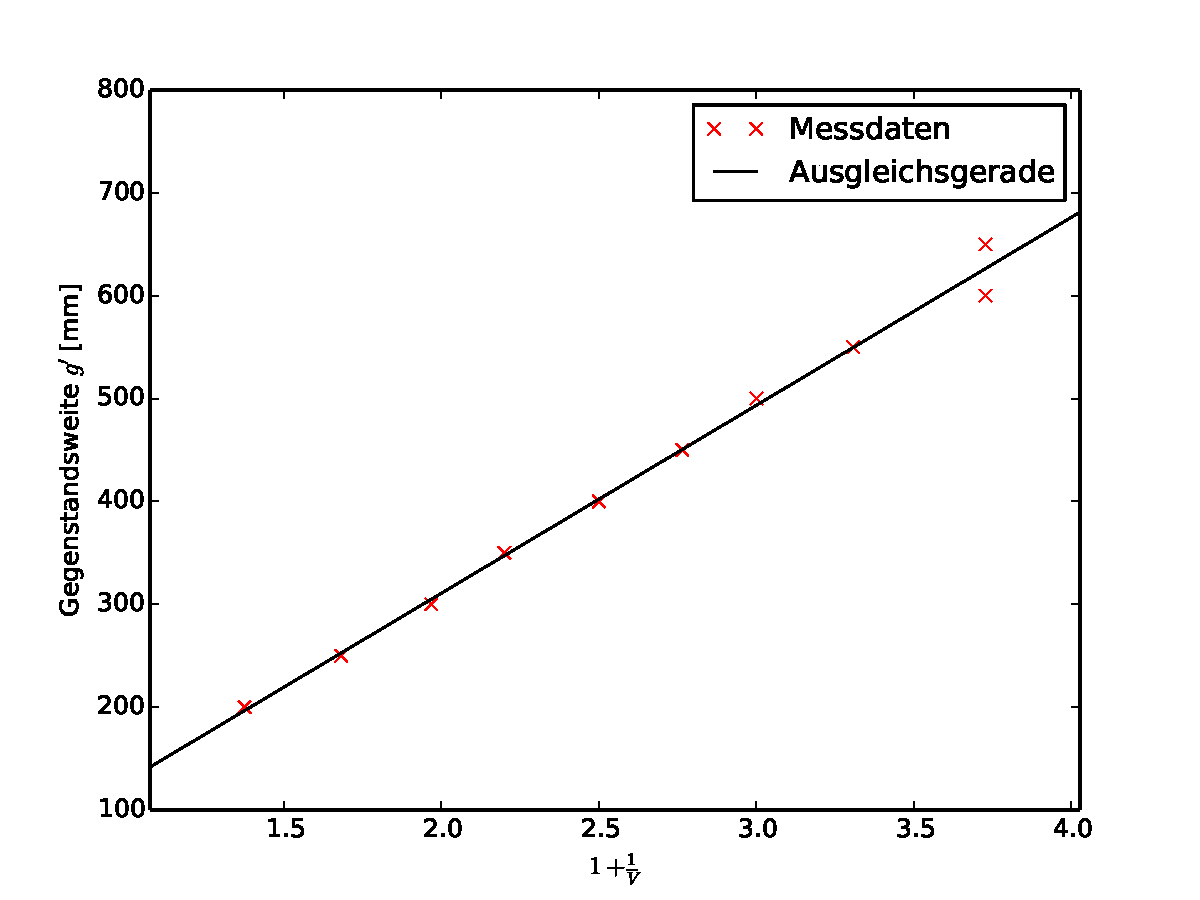
\includegraphics[width=0.8\textwidth]{Bilder/Abbe1.pdf}
	\caption{Messwerte für \texorpdfstring{\textsc{Abbe}}{Abbe}-Methode und Regression der Gleichung \eqref{eq:abbe1}. \cite{matplotlib}}
	\label{fig:abbe1}
\end{figure}
\begin{figure}[p]
	\centering
	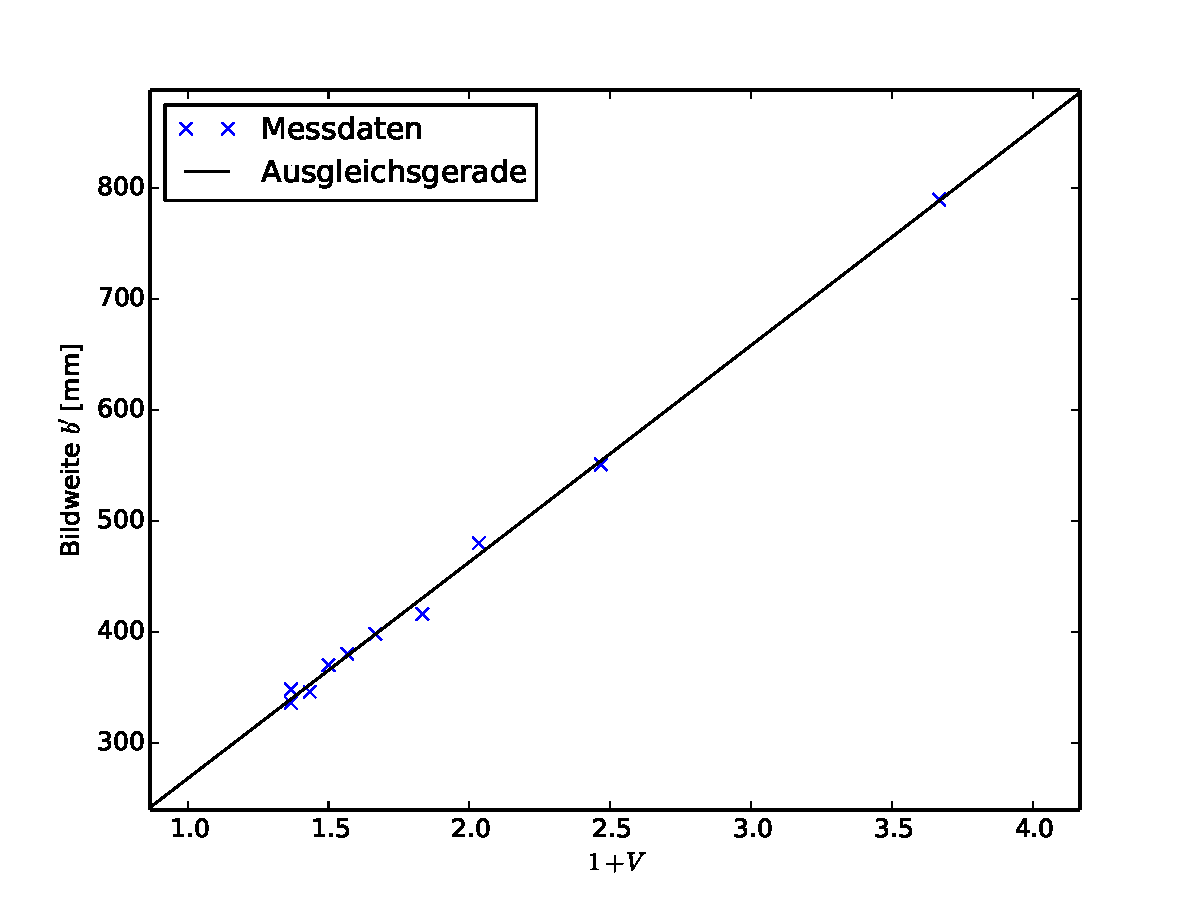
\includegraphics[width=0.8\textwidth]{Bilder/Abbe2.pdf}
	\caption{Messwerte für \texorpdfstring{\textsc{Abbe}}{Abbe}-Methode und Regression der Gleichung \eqref{eq:abbe2}.\cite{matplotlib}}
	\label{fig:abbe2}
\end{figure}